\documentclass{article}
\usepackage[utf8]{inputenc}
\usepackage{graphicx}

\title{Homework 10}
\author{Iman Tabrizian}
\date{March 2019}
\renewcommand\thesection{\Alph{section}}
\begin{document}

\begin{titlepage}
\maketitle
\end{titlepage}

\section{Identifying pilots + preambles (preamble equalizer present)}

\subsection{}

\begin{figure}[h]
    \centering
    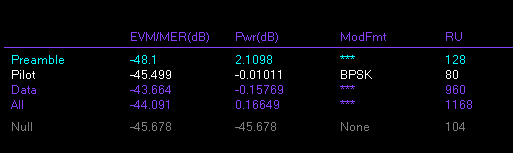
\includegraphics{data-burst-info}
    \caption{Data Burst Info}
\end{figure}

The total RU including the null is 1272.

\begin{itemize}
    \item \textbf{Preamble}: $128 / 1168 = 10.95 $ \%
    \item \textbf{Pilot}: $80 / 1168 = 6.84$ \%
    \item \textbf{Data}: $960 / 1168 = 82.19$ \%
\end{itemize}

\subsection{}

Figure 2 shows the OFDM symbols. VSA uses different colors for each of the preamble, pilot and data. For preamble it uses cyan, for pilot it uses white and for data it uses purple and green. The purple section is the part which is not changing which is the training sequence.

\begin{figure}[htb!]
    \centering
    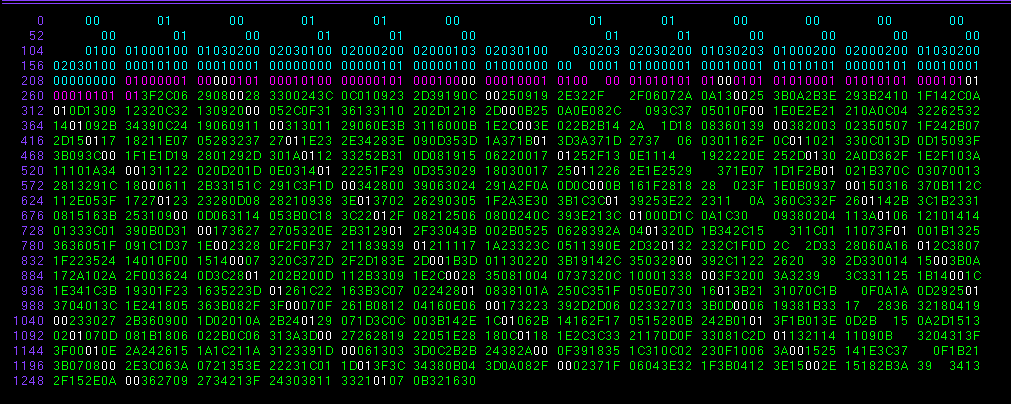
\includegraphics[scale=0.5]{symbols}
    \caption{OFDM Symbols}
\end{figure}

From the OFDM Meas we can see that there are 64 constellations (64-QAM). Figure 3 shows the constellation graph. Only carriers from -26 to 26 is being used. So, $64-52=12$ carriers are free. The pilots are on 21, -21, 7 and -7 carriers. The data and preamble are on the other remaining carriers.

\begin{figure}[htb!]
    \centering
    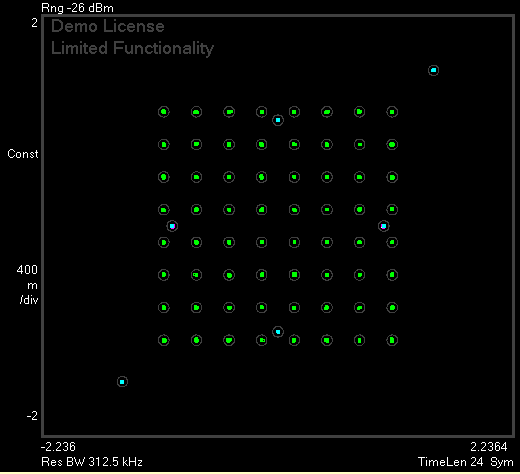
\includegraphics[scale=0.5]{ofdm-meas}
    \caption{Constellations}
\end{figure}

\subsection{}
You can find the constellation in figure 3. The figure 3 colors are like the question 2. The 6 cyan dots are preambles. The pilots are white and they are mixed with the green dots. 

\subsection{}
The purpose of using preamble is to provide synchronization for the receiver. Using preambles receiver can identify the beginning of other digital transmission. Pilots are used by the receiver to estimate Channel State Information. For example, amplitude and phase of each of sub carriers can be estimated using pilot tones. The training sequence at the beginning of the data is used for estimating CSI.

\section{Assessing performance (no equalizer)}

\begin{figure}[htb!]
    \centering
    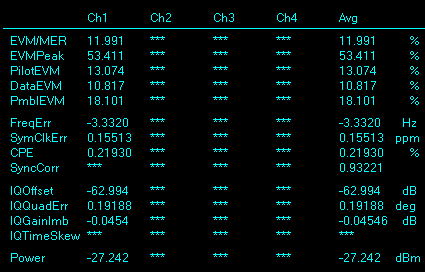
\includegraphics[scale=0.8]{error-summary}
    \caption{Error Summary}
\end{figure}

\subsection{Error Summary}
As you can see in the Figure 4, the average EVR/MER is 11.991 \%.

\subsection{Error Vector Summary}

Minimum and maximum EVM are shown in Figure 5 and results are in the table 1.

\begin{table}[htb!]
    \centering
    \begin{tabular}{|c|c|c|}
    \hline
             & Minimum EVM & Maximum EVM\\ \hline
         EVM & 1.8546 & 53.4112 \\ \hline
         sub-channel number & -18 & 24 \\ \hline
    \end{tabular}
    \caption{Error Vector Spectrum}
\end{table}

\begin{figure}[htb!]
    \centering
    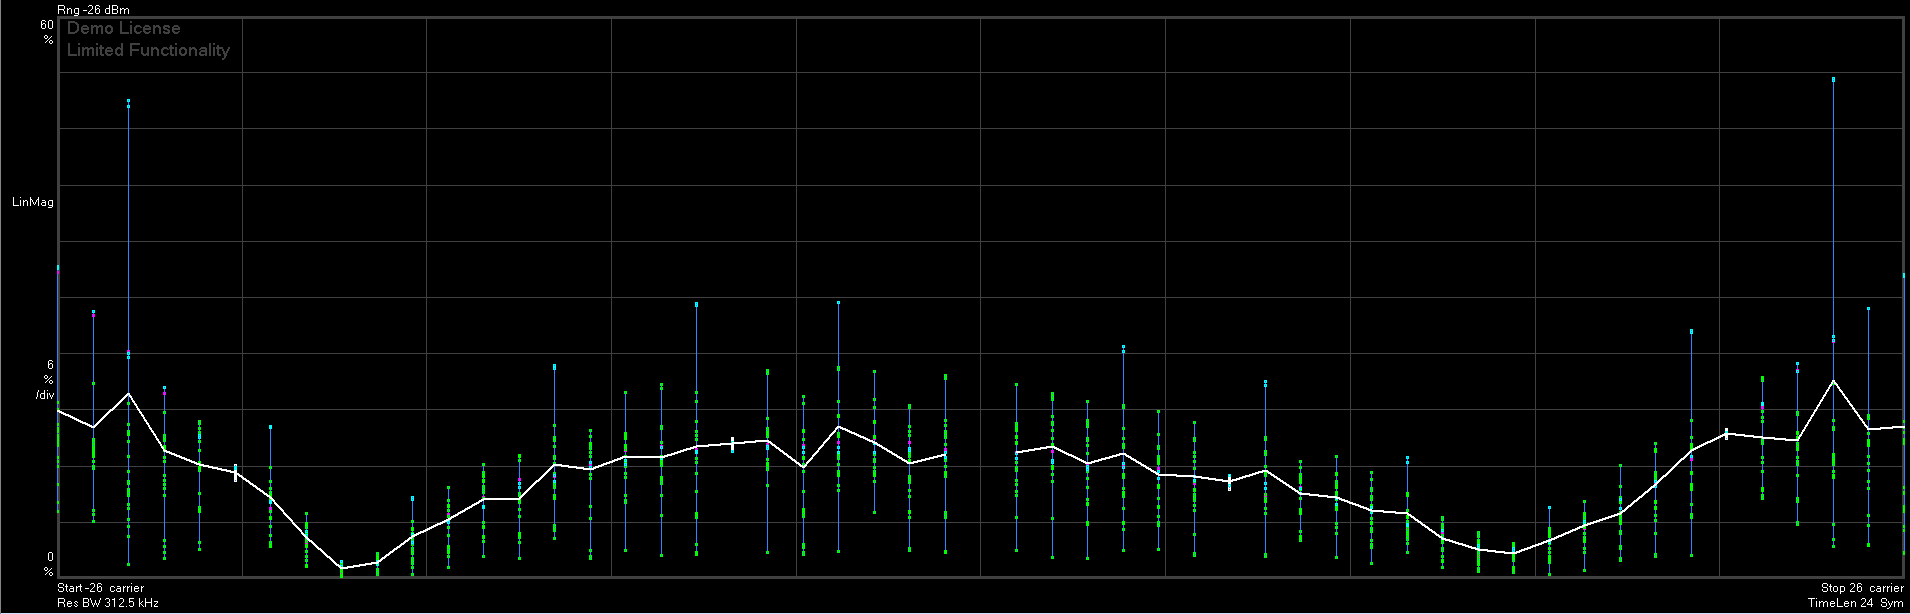
\includegraphics[scale=0.3]{error-vector-spectrum}
    \caption{Error Summary}
\end{figure}

\subsection{}
You can find the constellation diagram in the Figure 6. Compared to the Figure 3 the constellation diagram is more noisier. The dots are spread instead of being centered in a fixed point. Increase in the noise is also visible in the EVM compared to the signal with equalization.

\begin{figure}[htb!]
    \centering
    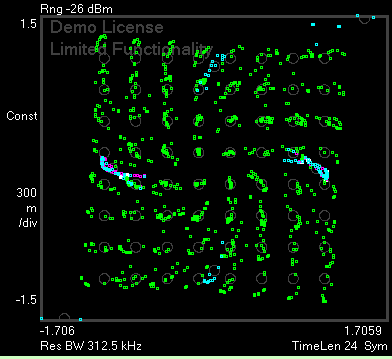
\includegraphics[scale=1]{ofdm-meas-2}
    \caption{Constellation without Equalizer}
\end{figure}

\section{Assessing performance (with various equalizers)}

\subsection{}
\begin{table}[htb!]
    \centering
    \begin{tabular}{|c|c|c|c|}
    \hline
         Equalizer & Pilot only & Preamble only & Data only \\ \hline
         Average EVM & 4.8019 \% & 0.62435 \% & 1.1747 \% \\ \hline
    \end{tabular}
    \caption{Error Vector Spectrum}
\end{table}

\subsection{}
\begin{figure}[htb!]
    \centering
    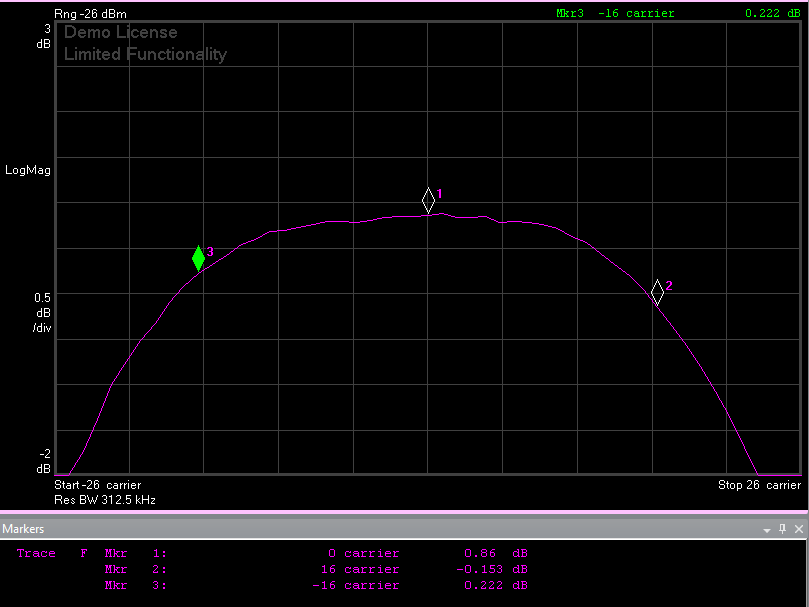
\includegraphics[scale=0.5]{ofdm-eq-ch-freq-resp}
    \caption{OFDM Eq Ch Freq Resp}
\end{figure}

Figure 7 shows the frequency response of the channel and the bandwidth measurements. The center frequency is at 5.804 GHz and the 3 dB bandwidth is about 9.3896 MHz on the right side and 9.4580 MHz on the left side.

\subsection{}
You can find the error vector spectrum in figure 8. As you can see average EVM is lower in compared with Figure 5. Additionally, variance is lower among different channels. It shows the role of equalizer in reducing both the mean and standard deviation of the EVM.

\begin{figure}[htb!]
    \centering
    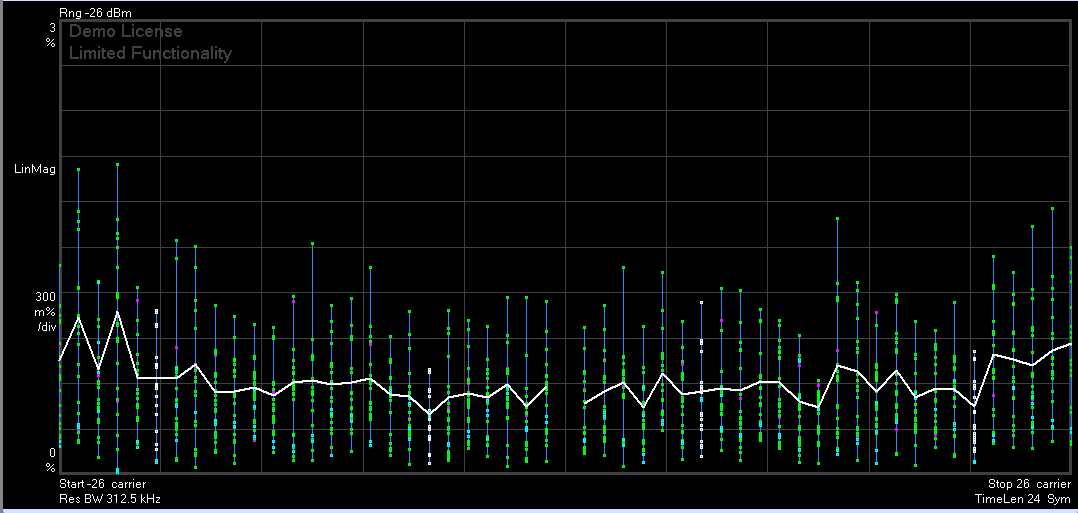
\includegraphics[scale=0.45]{error-vector-spectrum-new}
    \caption{Error Vector Summary}
\end{figure}

\section{Identifying spectrum parameters}
\subsection{}

4 sub channels are used in the question B.

\subsection{}
\begin{figure}[htb!]
    \centering
    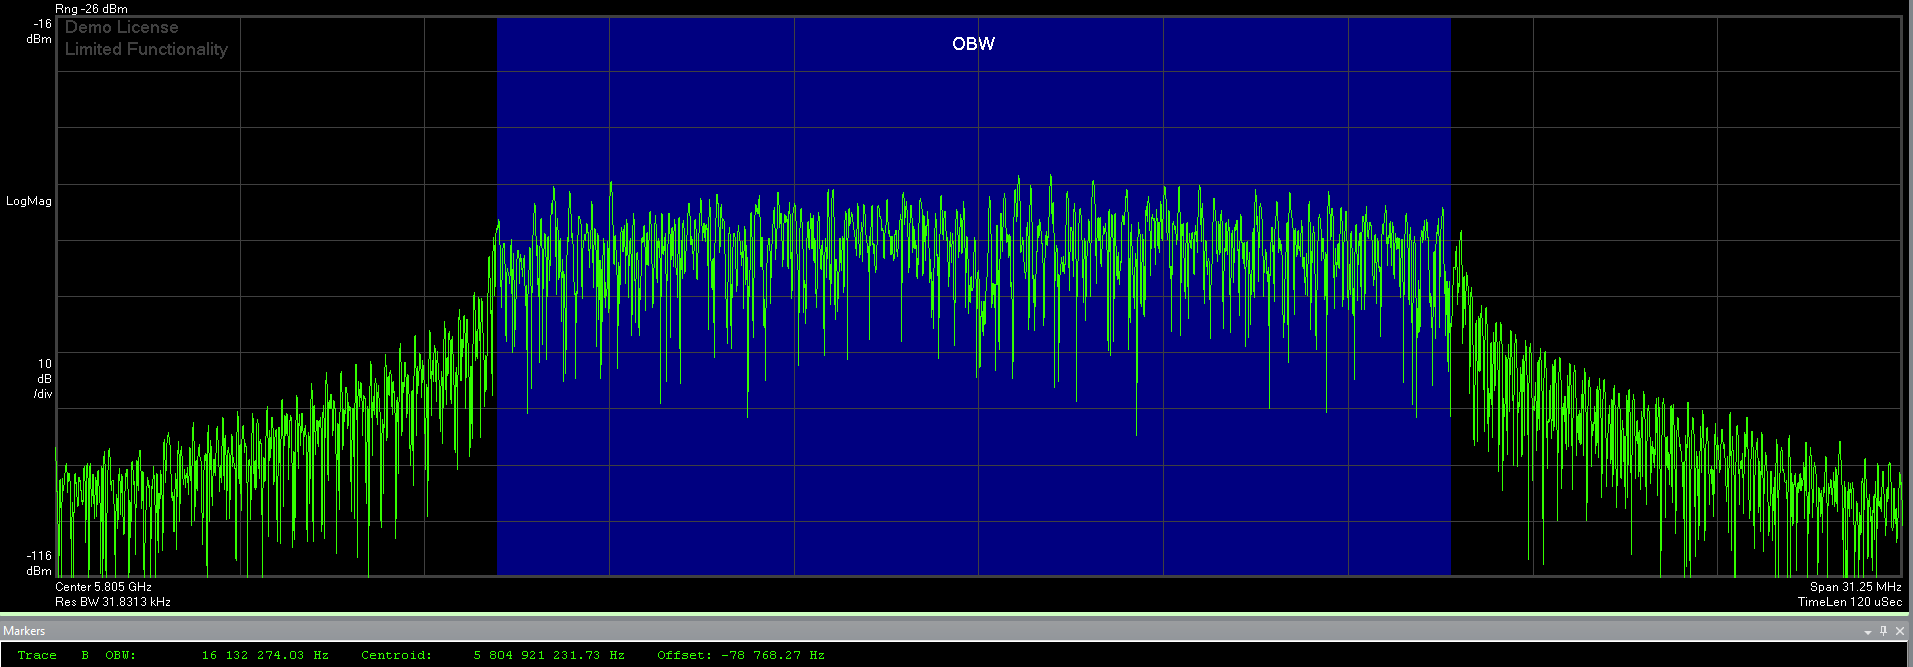
\includegraphics[scale=0.30]{obw-spectrum}
    \caption{Spectrum OBW}
\end{figure}

You can find the spectrum with OBW measurements in Figure 9. The bandwidth using OBW at 99\% power setting is 16.132 MHz.

\subsection{}
The FFT length is 64. With OBW of 16.132 MHz the guard band between sub channels is $20 - 16.132=3.868$.

\end{document}
